\documentclass[journal,10pt]{IEEEtran}

\makeatletter
\def\input@path{{./}{Paper/}}
\makeatother

% Optional math commands
\input{math_commands.tex}

\usepackage{times}
\usepackage[hypertexnames=false,hidelinks]{hyperref}
\usepackage{url}
\usepackage{booktabs}
\usepackage{amsmath,amssymb,amsfonts}
\usepackage{graphicx}
\usepackage{algorithm}
\usepackage{algorithmic}
\usepackage{color}
\usepackage[numbers,sort&compress]{natbib}
\usepackage{makecell}

% IEEEtran renders table captions in fake small-caps (\scshape), which at
% \footnotesize drops the visual size to ~6.4pt. Override the table-caption
% branch only: keep 8pt (\footnotesize) regular text, two-line IEEE style.
\makeatletter
\renewcommand{\@makecaption}[2]{%
  \ifx\@captype\@IEEEtablestring%
    \footnotesize\bgroup\par\centering\@IEEEtabletopskipstrut
      {\normalfont\footnotesize #1}\\{\normalfont\footnotesize #2}%
    \par\addvspace{0.5\baselineskip}\egroup%
    \@IEEEtablecaptionsepspace
  \else%
    \@IEEEfigurecaptionsepspace
    \setbox\@tempboxa\hbox{\normalfont\footnotesize {#1.}\nobreakspace\nobreakspace #2}%
    \ifdim \wd\@tempboxa >\hsize%
      \setbox\@tempboxa\hbox{\normalfont\footnotesize {#1.}\nobreakspace\nobreakspace}%
      \parbox[t]{\hsize}{\normalfont\footnotesize\noindent\unhbox\@tempboxa#2}%
    \else%
      \hbox to\hsize{\normalfont\footnotesize\box\@tempboxa\hfil}%
    \fi\fi}
\makeatother

% Path to figures (supports compiling from Paper/ or repo root)
\graphicspath{{./figures/}{Paper/figures/}}

\title{Texture Resonance Retrieval for Guitar-Effect Preset Selection}
\author{Anonymous Authors}

\begin{document}
\newcommand{\paperbibliostyle}{IEEEtranN}
\maketitle

\begin{abstract}
Digital audio workstations expose editable effect chains, but mapping user intent to low-level control parameters remains difficult because acoustic similarity does not always imply parameter transferability. We study editable guitar-effect control as parameter-transferability-aware executable neighborhood retrieval: a system should retrieve presets that are executable by the effect chain and useful as editable parameter starting points. We propose Texture Resonance Retrieval (TRR), which leverages mid-level Wav2Vec2 activations and captures their stationary texture structure via second-order Gram statistics. On an audited 204-query pilot benchmark with 1,063 candidate presets, TRR achieves the best full-coverage top-1 retrieval result among evaluated baselines, reducing normalized parameter distance from 0.1960--0.2002 to 0.1454. Mechanism ablations indicate that this gain is coupled with the choice of mid-level layer 5; we therefore frame TRR as a texture-aware retrieval prior using mid-level deep features, rather than as a claim about second-order statistics in isolation. We further introduce exemplar-preserving projection (EPR-K5), a constrained projection over retrieved neighbors that improves TRR to 0.1334 normalized distance while retaining neighborhood provenance. A range-projected MLP is retained as a supervised direct-regression boundary: it nearly ties TRR EPR-K5 on normalized tolerance (Acc@0.1=0.7894 vs. 0.7908) but lacks retrieved-neighborhood provenance and is substantially weaker on normalized distance, recall, and cosine similarity. This comparison clarifies that the core advantage of TRR is not numerical precision on a single tolerance metric but rather the editable provenance and full-parameter alignment that retrieval over real exemplars provides. Leakage, hard-split, degraded-input, and listening diagnostics bound the claim to the current guitar-effect benchmark.
\end{abstract}

\begin{IEEEkeywords}
guitar-effect preset retrieval, audio retrieval, digital audio workstations, texture representation, interpretable audio systems
\end{IEEEkeywords}

\section{Introduction}
\label{sec:introduction}

	The field of neural audio synthesis currently faces a fundamental tension between \textit{fidelity} and \textit{control}. Recent high-fidelity generative models, primarily based on latent diffusion \citep{liu2023audioldm,agostinelli2023musiclm}, can achieve strong perceptual quality but often operate as ``black boxes.'' They generate finalized waveforms where internal attributes—such as the attack time of a compressor or the decay of a reverb—are entangled and inaccessible for post-hoc editing. Conversely, Differentiable Digital Signal Processing (DDSP) \citep{engel2020ddsp} offers interpretable, structured control but often suffers from the ill-posed nature of the inverse parameter estimation problem.

This tension motivates the development of retrieval-based audio control systems that can map user intent to interpretable DSP parameters. By retrieving relevant presets rather than generating parameters from scratch, such systems are designed to produce editable outputs that integrate with DAW workflows. In this view, retrieval is valuable not because it solves the inverse problem in closed form, but because it places the query in a plausible executable neighborhood of parameter space that the user can still inspect and refine.

The key challenge is grounding user descriptions in parameter space via retrieval. Standard audio representations (e.g., CLAP-style embeddings or mean-pooled Wav2Vec2 features) summarize an audio segment into a single vector; while effective for coarse semantics, such pooling can discard temporal co-activation patterns that are critical for texture-dominant effects (e.g., tremolo modulation or signal-dependent distortion).

To bridge these gaps, we study a retrieval-grounded preset-selection setting and focus on its core retrieval component: \textbf{Texture Resonance Retrieval (TRR)}. TRR models audio style using Gram matrices of deep feature activations, explicitly capturing the correlation structure that defines temporal texture. We use this representation as a texture-aware retrieval prior that biases search toward executable presets with preserved effect-relevant structure. We evaluate TRR on a curated guitar-effect preset benchmark of 1,063 candidates and 204 held-out queries.

Concretely, this paper makes four evidence-bounded contributions. First, we formulate editable guitar-effect control as parameter-transferability-aware executable neighborhood retrieval, distinguishing it from waveform generation, general semantic retrieval, and direct parameter regression. Second, we evaluate TRR as a texture-aware retrieval prior built on mid-level deep features; we report second-order Gram statistics as an effective aggregation operator and use controlled ablations to clarify that the advantage is coupled with mid-level layer selection. Third, we add Top-K neighborhood and exemplar-preserving projection diagnostics to measure whether retrieval places a query in a useful editable preset neighborhood rather than only optimizing top-1 similarity. Fourth, we report an audited evaluation package including Protocol-A retrieval, near-duplicate filtering, parameter-cluster hard split, direct-regression boundary, multimodal degradation diagnostics, and exploratory listening evidence.

\section{Related Work}
\label{sec:related_work}

Our work lies at the intersection of intelligent music production, neural audio synthesis, audio representation learning, and retrieval-grounded parameter control. Semantic control of audio effects has long been studied in intelligent music production, including semantic-to-parameter mapping in DAW settings \citep{stables2014semantic}, interactive control learning \citep{huang2014active}, and recent multimodal synthesizer retrieval tools \citep{bryan2024synthscribe}. These systems motivate editable parameter control, but they do not directly address whether retrieved presets form parameter-transferable neighborhoods under auditable held-out protocols. The SAFE project \citep{stables2014semantic} established semantic audio descriptors for retrieval, yet its descriptors are human-annotated first-order labels rather than learned second-order texture statistics, and its evaluation does not report parameter-space transferability on held-out splits. Recent automixing and parameter-optimization systems \citep{steinmetz2022automix,moliner2025megami,benetos2024stito} optimize effect chains via gradient descent or Bayesian methods, yielding strong numerical results but producing dense parameter vectors without exemplar provenance. We position TRR as a retrieval-based alternative that guarantees executability and preserves editability by anchoring outputs to real preset exemplars.

Neural audio synthesis and differentiable DSP provide complementary foundations. Text-to-audio and latent-diffusion systems \citep{liu2023audioldm,agostinelli2023musiclm,liu2024audioldm2} generate high-quality waveforms, while DDSP-style methods \citep{engel2020ddsp,peladeau2024blind,liu2024ddspSFX} and neural emulation of analog audio circuits \citep{wright2020realtime} expose more structured controls. Recent work further pursues large-scale synthetic augmentation and contrastive learning for guitar-effects encoders \citep{wright2024openamp}, though evaluation has focused on classification accuracy rather than parameter-space retrieval on held-out presets. Recent intelligent music production systems also pursue direct parameter control: LLM2Fx \citep{doh2025llm2fx} predicts audio effect parameters from natural language, and ST-ITO \citep{benetos2024stito} optimizes effect parameters via inference-time gradient descent. These approaches regress or optimize parameters without exemplar provenance. Human--computer interaction studies with practising musicians confirm that editability, provenance, and DAW integration are decisive adoption factors for creative AI tools \citep{fiebrink2009wekinator,krol2025codesign,tchemeube2023mmmc}. Our target is different: rather than synthesizing final audio or regressing parameters without provenance, we retrieve executable presets that remain inspectable and editable in downstream DAW workflows. Retrieval trades some optimality for guaranteed feasibility and human-readable provenance.

Modern audio encoders such as CLAP \citep{elizalde2023clap}, PaSST \citep{koutini2022passt}, PANNs \citep{kong2020panns}, and Wav2Vec2 \citep{baevski2020wav2vec} provide strong first-order or semantic embeddings. However, perceptual similarity does not necessarily imply parameter transferability for effect-chain control. Inspired by Gram-matrix style representations \citep{gatys2015style,ulyanov2016audio} and audio texture analysis \citep{stylianou2015audio,mcwec2023texture}, TRR uses second-order deep-feature statistics as a retrieval descriptor for executable preset selection. This connects to a broader literature on audio texture perception and synthesis, where stationary statistical properties of the auditory periphery have been shown to characterize texture identity \citep{mcdermott2011sound}. In contrast to document-centric retrieval-augmented generation \citep{lewis2020rag} or open-ended music generation, the retrieval target here is a finite set of valid parameter exemplars, and success is measured in parameter space with explicit coverage, leakage, and validity audits.

\section{Problem Formulation}
\label{sec:problem_formulation}

We formalize audio-effect preset selection as constrained retrieval over executable parameters. Let $\Phi:\mathcal{X}\times\Theta\rightarrow\mathcal{X}$ denote a DSP rendering operator and let $\Theta\subset\mathbb{R}^{d}$ denote the parameter space of a multi-effect guitar processing chain. The feasible set is bounded and structurally constrained:
\begin{equation}
    \label{eq:feasible_set}
    \Theta = \left\{ \theta \in \mathbb{R}^d \mid \mathbf{l} \preceq \theta \preceq \mathbf{u}, \quad \mathcal{C}(\theta) = 1 \right\}
\end{equation}
where $\mathcal{C}$ encodes plugin-specific validity constraints. Given a query $q=(t,\mathbf{a}_{\mathrm{ref}})$, containing a text description and optionally an audio reference, the objective is to return a valid, editable parameter vector:
\begin{equation}
	\tilde{\theta} \in \Theta \quad \text{given } q,
\end{equation}
where query consistency is operationalized through parameter-space evaluation against held-out presets. Because the inverse mapping from user intent to parameters is ill-posed and the DSP validity constraints are strict, we retrieve a top-$K$ executable neighborhood from a finite preset database:
\begin{equation}
	\theta_{\text{selected}} = \text{Top-}K(q)
\end{equation}
Retrieval supplies a mode-seeking step that places the query in a plausible neighborhood of $\Theta$; projection and validity repair then operate only within this retrieved support. This framing distinguishes our task from unconstrained waveform generation and from direct dense parameter regression without exemplar provenance.

\section{Methodology}
\label{sec:methodology}

We implement the retrieval-based framework defined in Section \ref{sec:problem_formulation} via \textbf{Texture Resonance Retrieval (TRR)} to retrieve candidate presets using texture statistics derived from mid-level deep features.

\subsection{System Architecture}
\label{ssec:architecture}

The system realizes $\Phi(\mathbf{x}_{\text{in}};\theta)$ through a decoupled design over a switchable nine-module topology: Compressor $\to$ Driver $\to$ Screamer $\to$ Equaliser $\to$ Chorus $\to$ Flanger $\to$ Phaser $\to$ Delay $\to$ Reverb.

The architecture has two components. The real-time DSP engine executes validated parameters as a deterministic audio graph. The retrieval module runs asynchronously from the audio callback, maps $q$ to candidate presets, and returns parameters only after validity checking. This separation keeps the submitted method focused on retrieval quality rather than claiming unverified real-time inference.

\subsection{Texture Resonance Retrieval (TRR)}
\label{ssec:rag}

The core challenge in texture-aware retrieval lies in computing a similarity metric for the audio modality that preserves effect-relevant dynamics. Standard embeddings (e.g., mean-pooled Wav2Vec2 features) collapse temporal structure into a static vector, losing information that is critical for effects like modulation and distortion.

To address this, we introduce \textbf{Texture Resonance Retrieval (TRR)}. Drawing on the hypothesis that audio texture is encoded in second-order feature statistics \citep{mcdermott2011sound}, we compute the Gram matrix of deep activations. In our formulation, \textit{texture} refers to stationary statistical properties of the audio signal that are invariant to exact temporal alignment, as distinct from \textit{timbre} (spectral envelope of individual events) or \textit{style} (higher-level genre semantics).

\begin{algorithm}[ht]
		\caption{TRR Encoding}
		\label{alg:trr_encoding}
		\begin{algorithmic}
			\REQUIRE Audio sample $a$, Wav2Vec2 model $\mathcal{W}$, layer set $\mathcal{L}=\{4,5,6\}$, frozen random linear projection $P:\mathbb{R}^{768}\rightarrow\mathbb{R}^{64}$
			\ENSURE Texture embedding $\mathbf{g}_{\text{norm}}$

			\STATE \textbf{1. Preprocessing}: Normalize $a$ and pad to minimum length.
			\FOR{each $\ell \in \mathcal{L}$}
			\STATE $\mathbf{H}_{\ell} \leftarrow \mathcal{W}_{\text{layer }\ell}(a) \in \mathbb{R}^{T_{\text{frm}} \times 768}$
			\STATE $\widehat{\mathbf{H}}_{\ell} \leftarrow P(\mathbf{H}_{\ell}) \in \mathbb{R}^{T_{\text{frm}} \times 32}$ \COMMENT{Frozen; Xavier init. used only for initial variance scaling}
			\STATE $\mathbf{G}_{\ell} \leftarrow \frac{1}{T_{\text{frm}}}\widehat{\mathbf{H}}_{\ell}^{\top}\widehat{\mathbf{H}}_{\ell} \in \mathbb{R}^{32 \times 32}$
			\ENDFOR
			\STATE $\bar{\mathbf{G}} \leftarrow \frac{1}{|\mathcal{L}|}\sum_{\ell\in\mathcal{L}}\mathbf{G}_{\ell}$
			\STATE $\mathbf{g}_{\text{norm}} \leftarrow \mathrm{vec}(\bar{\mathbf{G}}) / \|\mathrm{vec}(\bar{\mathbf{G}})\|_2$
		\RETURN $\mathbf{g}_{\text{norm}}$
	\end{algorithmic}
\end{algorithm}

Let $\mathbf{H}_{\ell} \in \mathbb{R}^{T_{\text{frm}} \times 768}$ be the frame-level activation map from layer $\ell$ of a pre-trained Wav2Vec2 Base model. In the benchmarked implementation we use the mid-level layer set $\mathcal{L}=\{4,5,6\}$, apply a frozen Xavier-initialized random projection to 64 dimensions, compute a Gram matrix per layer, average the resulting $64\times 64$ matrices, flatten the result into a 4096-dimensional vector, and L2-normalize it. The averaged texture descriptor can be written as
\begin{equation}
		\bar{\mathbf{G}} = \frac{1}{|\mathcal{L}|}\sum_{\ell\in\mathcal{L}} \frac{1}{T_{\text{frm}}}\widehat{\mathbf{H}}_{\ell}^{\top}\widehat{\mathbf{H}}_{\ell},
\end{equation}
where $\widehat{\mathbf{H}}_{\ell}$ denotes the projected feature map. The entry $\bar{\mathbf{G}}_{ij}$ captures the co-activation of projected channels $i$ and $j$ irrespective of their absolute temporal position. This time-invariance allows TRR to match textures (e.g., ``fast tremolo'') even if the reference and database entries are not phase-aligned. L2 normalization of $\mathrm{vec}(\bar{\mathbf{G}})$ is equivalent to Frobenius normalization of the matrix representation, and similarity is then computed as cosine similarity between the flattened descriptors. Computationally, Gram-matrix construction scales as $O(D^2 \cdot T_{\text{frm}})$ after projection, where $D=64$ in the reported implementation. This bound covers only the post-Wav2Vec2 Gram construction; the Wav2Vec2 forward pass is a separate feature-extraction cost and dominates when features are not cached.

TRR is a second-order summary of deep features: it retains cross-channel correlation structure while discarding absolute temporal alignment. For a frame permutation matrix $\mathbf{P}$, $(\mathbf{P}\mathbf{H})^\top(\mathbf{P}\mathbf{H})=\mathbf{H}^\top\mathbf{H}$, so Gram aggregation is insensitive to frame order. This property is useful for effect textures whose perceptual identity depends on stationary co-activation patterns rather than exact temporal alignment. Figure~\ref{fig:representation_diagnostics} visualizes the resulting representation at two levels: an example Gram matrix that exposes the co-activation structure used by TRR, and a t-SNE diagnostic comparing TRR with mean-pooled Wav2Vec2 embeddings. These plots are interpretive diagnostics; the quantitative claim remains anchored to the held-out Protocol-A/Protocol-B metrics.

\begin{figure*}[t]
\centering
\begin{minipage}{0.34\textwidth}
	\centering
	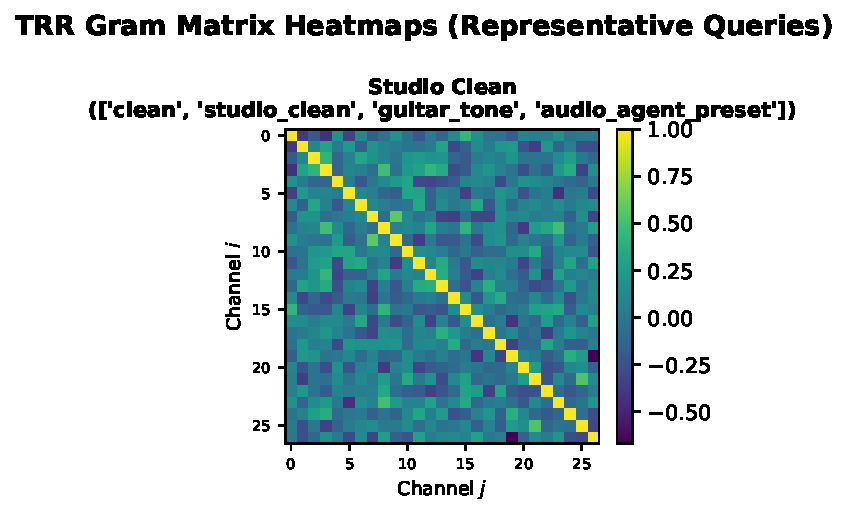
\includegraphics[width=\linewidth]{gram_matrix_examples.pdf}
	(a)
\end{minipage}
\hfill
\begin{minipage}{0.62\textwidth}
	\centering
	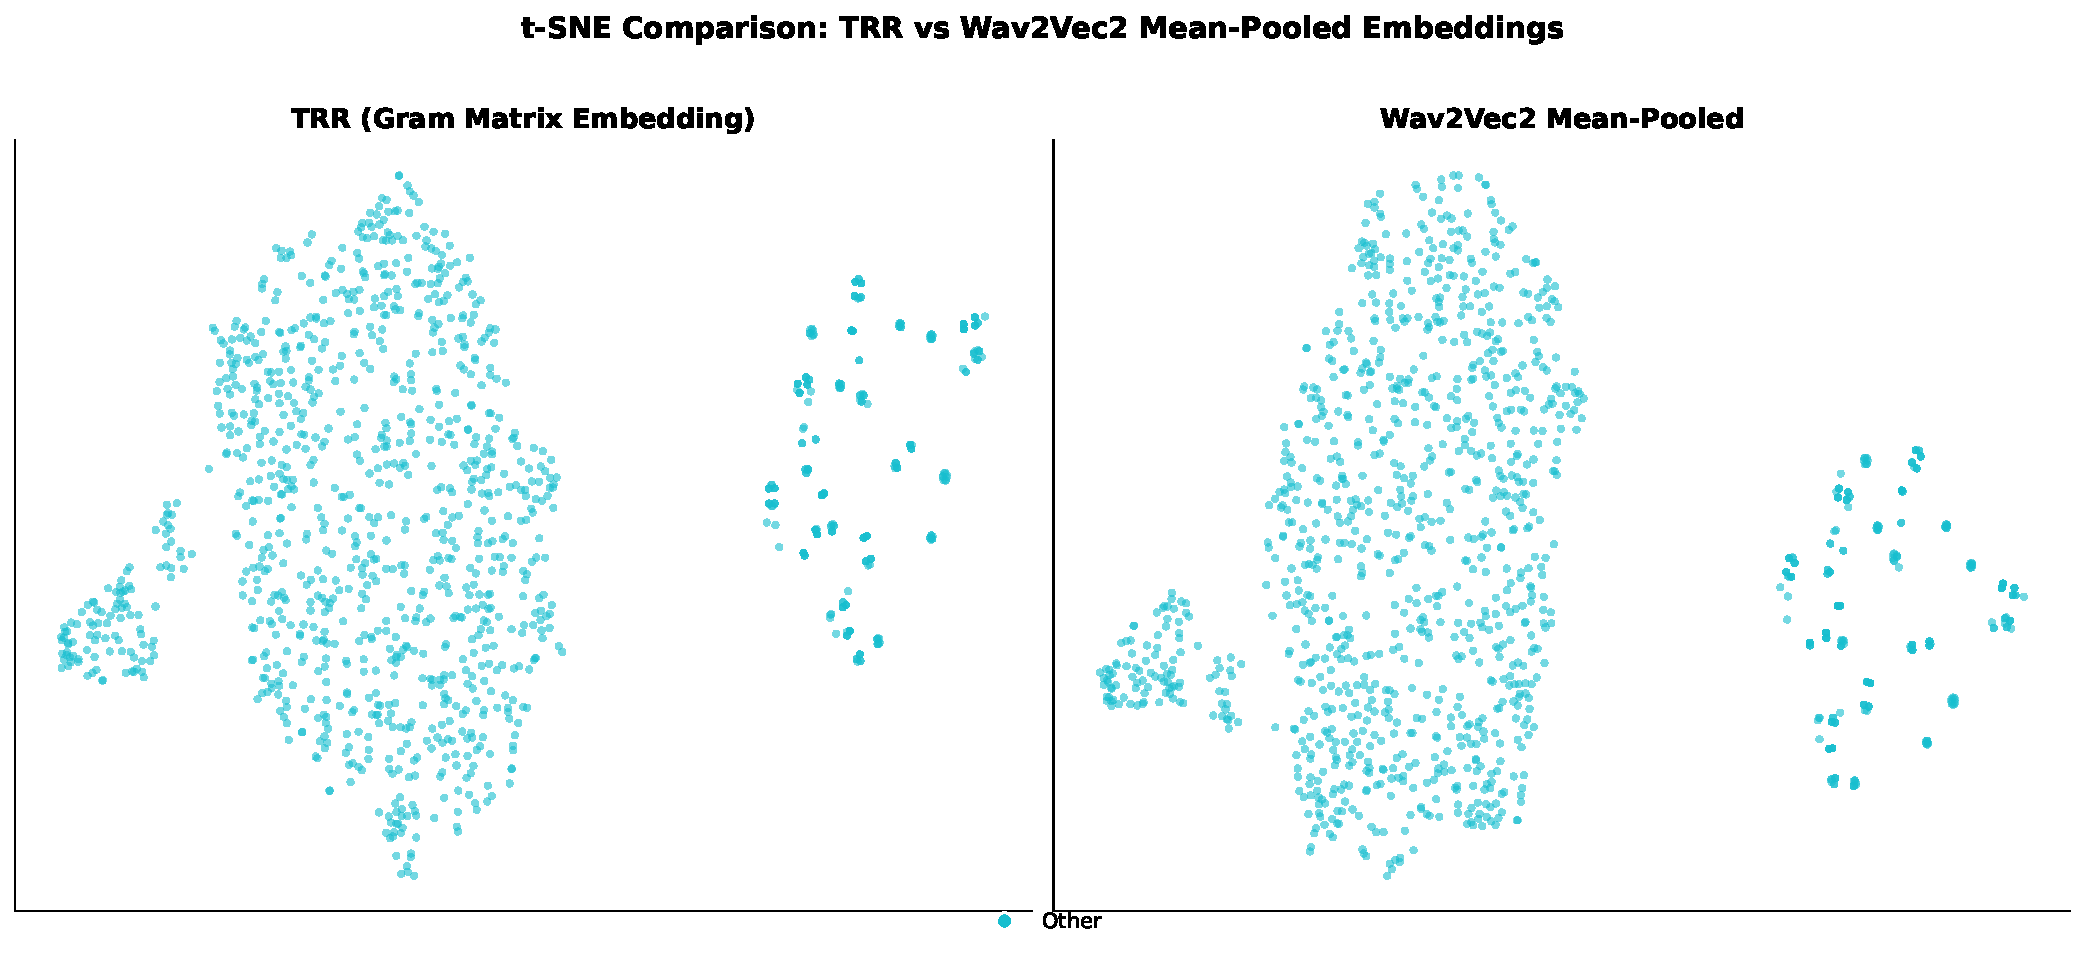
\includegraphics[width=\linewidth]{trr_vs_wav2vec_tsne.pdf}
	(b)
\end{minipage}
\caption{TRR representation diagnostics. (a) Example second-order Gram matrix. (b) t-SNE comparison between TRR and mean-pooled Wav2Vec2 embeddings on the benchmark presets. The figure is used for qualitative inspection rather than as standalone evidence of parameter transferability.}
\label{fig:representation_diagnostics}
\end{figure*}

\subsection{Protocol-B: Exemplar-Preserving Projection}
\label{ssec:epr}

Top-1 retrieval returns an executable preset, but it is unnecessarily brittle when several nearby presets form a more parameter-transferable neighborhood. We therefore introduce \textbf{Exemplar-Preserving Projection (EPR-K5)} as the Protocol-B module. Given a query $q$, a retrieval prior returns a top-$K$ executable neighborhood
\begin{equation}
	\mathcal{N}_K(q)=\{(\theta_i,s_i)\}_{i=1}^{K},
\end{equation}
where $\theta_i$ is a stored executable preset and $s_i$ is the retrieval similarity score. We fix $K=5$ and temperature $\tau=0.05$ for all methods and do not tune these hyperparameters on test labels. The exemplar weights are
\begin{equation}
	w_i=\frac{\exp(s_i/\tau)}{\sum_{j=1}^{K}\exp(s_j/\tau)}.
\end{equation}
For continuous numeric leaves, EPR computes a weighted average and clips each leaf to the observed range in the knowledge base:
\begin{equation}
	\tilde{\theta}_{\mathrm{cont}}=
	\Pi_{\Theta}\left(\sum_{i=1}^{K}w_i\theta_{i,\mathrm{cont}}\right).
\end{equation}
For binary module switches, EPR uses a weighted vote over the top-$K$ candidates and activates a switch when its weighted support exceeds $0.5$:
\begin{equation}
	\tilde{\theta}_{\mathrm{on}}=
	\mathbb{I}\left[\sum_{i=1}^{K}w_i\theta_{i,\mathrm{on}}>0.5\right].
\end{equation}
Missing keys are not artificially generated; as in the evaluator, missing numeric leaves enter the union-key metric as zeros. This keeps Protocol-B comparable with Protocol-A and avoids silently adding parameters that no retrieved exemplar supplies. We report provenance with the largest exemplar contribution $\max_i w_i$ and the inverse-Herfindahl effective exemplar count
\begin{equation}
	N_{\mathrm{eff}}=\frac{1}{\sum_{i=1}^{K}w_i^2}.
\end{equation}
EPR-K5 produces a new parameter vector that is not itself a stored preset: it is a softmax-weighted blend of retrieved exemplars followed by range and switch projection. Its output remains executable because every parameter value is either clipped to the observed range of retrieved neighbors or decided by a weighted vote over them. The neighborhood provenance ($N_{\mathrm{eff}}$ and $\max_i w_i$) documents which retrieved presets contributed, but the final vector is a synthetic projection rather than a single retrieved exemplar.

\subsection{Complexity and Latency}
\label{ssec:complexity_latency}
TRR encoding includes Wav2Vec2 feature extraction, then $O(D^2T_{\mathrm{frm}})$ Gram construction after projection with $D=64$, followed by top-$K$ nearest-neighbor search. Cached retrieval scoring is lightweight in the local artifact, but uncached live reference-audio latency is not claimed in the main paper because the reviewed artifact does not expose a complete live Wav2Vec2-forward profiling path.

\section{Experiments}
\label{sec:experiments}

We validate the proposed framework by answering one core research question: does modeling texture with mid-level deep-feature statistics (TRR) improve parameter inference compared to first-order baselines?

\subsection{Experimental Setup}

\paragraph{Dataset and Knowledge Base.}
The benchmark corpus contains 1267 paired records (audio--text--parameter triplets) collected from guitar effect presets. A post-hoc audit of the original song-name-based held-out list (211 test queries, 1056 knowledge-base items) revealed 16 cross-split shared resolved audio paths and 48 near-duplicate cross-split pairs under a cheap fingerprint. To remove exact audio reuse from the main objective benchmark, we regroup records by resolved local audio path before sampling the held-out set. The resulting stricter Protocol-A split contains 204 test queries and 1063 knowledge-base items, with zero exact shared resolved audio paths across split under the current audit. We retain this as a pilot benchmark because cheap near-duplicate pairs remain and the corpus is still guitar-only.

\paragraph{Provenance notes.}
The dataset JSON exposes song name, style tags, feature tags, parameters, and stored vectors, but it does not include a separate auditable text-source field. We therefore treat the style and feature fields as the only explicit text-side provenance available in-repo, and use the stored parameters as the operational ground truth.

\paragraph{Scope and protocol.}
Unless otherwise stated, objective results in this section use \textbf{Protocol-A} for top-1 retrieval and \textbf{Protocol-B} for executable-neighborhood projection on the same 204-query split and the same 1,063-record retrieval database. Protocol-C, listening tests, and latency measurements are reported on their own protocol-specific pools and are labeled explicitly.

\paragraph{Resources and reproducibility.}
\label{sec:repro}
To facilitate reproducibility, the supplementary package contains preprocessing details, embedding computation steps, retrieval-index construction, prompt templates, evaluation scripts, and split specifications for all reported tables. The artifact package is anonymized for review and is intended to make each reported table traceable to a script-level evidence path.

\paragraph{Baselines.}
We compare our proposed \textbf{TRR} (Section \ref{ssec:rag}) against locally auditable retrieval baselines. \textbf{Wav2Vec} uses mean-pooled Wav2Vec2 activations. \textbf{FeatureNN} uses the released benchmark feature vectors and should therefore be interpreted as a fixed dense-retrieval reference. \textbf{CLAP} uses the stored CLAP vectors available in the local JSON artifact and is reported with its actual coverage. \textbf{PaSST} is regenerated in the E9 derived artifact with full Protocol-A coverage and serves as the full-coverage modern audio-encoder baseline. PANNs remains excluded from unified tables because its local Python 3.12 inference path fails through the \texttt{librosa}/\texttt{numba} dependency chain; we therefore do not claim a fair PANNs EPR baseline.

\subsection{Metrics}
\label{ssec:metrics}
We evaluate alignment in parameter space $\Theta$ using operational metrics computed on flattened numeric parameter leaves. Concretely, given a nested parameter dictionary, we recursively flatten numeric leaves into a sparse vector indexed by dot-separated keys (e.g., \texttt{DelayOn.Mix}) and ignore non-numeric leaves (e.g., strings). Unless otherwise stated, we form the union of keys between prediction and ground truth, and treat missing numeric keys as zeros for metric computation. The unified main table reports normalized L2, normalized Acc@0.1, Recall, Cosine, value-aware SwitchF1, coverage, and provenance. The earlier key-presence Module Jaccard is retained only as an audit diagnostic because it can reward methods that emit a complete schema even when switch values are not aligned. Raw L2 magnitudes can be dominated by a small number of large-scale parameters and are therefore retained only in protocol-specific audit artifacts. Normalized L2 uses plugin-defined min--max ranges for comparability, but this is still an engineering normalization rather than a perceptual scale: logarithmic, dB, and nonlinear control laws can make equal normalized parameter differences perceptually unequal.

\paragraph{L2 Error (RMSE).}
Given flattened vectors $v(\theta_{\text{gt}})$ and $v(\tilde{\theta})$ over the union key set of size $d$, we report the root mean squared error
\begin{equation}
	\text{L2} = \sqrt{\frac{1}{d}\sum_{i=1}^{d}\left(v(\theta_{\text{gt}})^{(i)} - v(\tilde{\theta})^{(i)}\right)^2}.
\end{equation}

\paragraph{Normalized Accuracy@0.1.}
For the unified tables, we report the fraction of normalized flattened numeric parameters whose absolute error is within a fixed tolerance $\tau=0.1$:
\begin{equation}
	\text{Norm.Acc@0.1} = \frac{1}{d}\sum_{i=1}^{d}\mathbb{I}\left(\left|v(\theta_{\text{gt}})^{(i)} - v(\tilde{\theta})^{(i)}\right| \leq 0.1\right).
\end{equation}

\paragraph{Recall (active numeric parameters).}
We define a ground-truth numeric parameter as \emph{active} if $\left|v(\theta_{\text{gt}})^{(i)}\right|>0.05$. Recall is the fraction of active ground-truth dimensions whose predicted value falls within the same tolerance $\tau=0.1$.

\paragraph{Cosine Similarity.}
We compute cosine similarity between flattened vectors over the union key set:
\begin{equation}
		\text{Cosine} = \frac{v(\theta_{\text{gt}})\cdot v(\tilde{\theta})}{\|v(\theta_{\text{gt}})\|_2\,\|v(\tilde{\theta})\|_2}.
\end{equation}

\paragraph{Switch-State Metrics.}
We report value-aware active-switch precision, recall, and F1 rather than using key presence alone. For each switch root, the evaluator infers the active state from the numeric \texttt{On}/\texttt{Off} leaves and compares the predicted active-switch set $S_{\text{pred}}$ against the ground-truth set $S_{\text{gt}}$:
\begin{equation}
	\text{SwitchF1} = \frac{2|S_{\text{gt}}\cap S_{\text{pred}}|}{|S_{\text{gt}}|+|S_{\text{pred}}|}.
\end{equation}
The legacy Module Jaccard over keys ending with \texttt{On} is still written to the audit JSON, but it is not used as a main evidence column.

\paragraph{Parameter-Neighborhood Recall.}
Because the task is executable-neighborhood retrieval rather than only top-1 nearest-preset selection, we also report parameter-neighborhood recall:
\begin{equation}
	\mathrm{PNR@K}=
	\mathbb{I}\left[\min_{i\in\mathrm{TopK}(q)}d_\theta(\theta_i,\theta_q)<\tau_p\right],
\end{equation}
where $d_\theta$ is normalized parameter RMSE. The primary table uses $\tau_p=0.10$ and the supplementary audit reports $\tau_p\in\{0.05,0.10,0.15\}$ sensitivity.

\subsection{Protocol-A: Comparative Retrieval Evaluation}
\label{ssec:protocolA}

\textbf{Purpose.} Benchmark top-1 executable retrieval and Protocol-B exemplar-preserving projection under one evaluator, one split, and one normalization path.

\textbf{Protocol.} Protocol-A uses top-1 retrieval on a deterministic 204-query test split and a 1,063-record retrieval database. Protocol-B applies the EPR-K5 projection defined in Section~\ref{ssec:epr} to the same retrieved neighborhoods. Both protocols use the same split, evaluator, normalized parameter distance, missing-key convention, and coverage accounting. A method is reported with its actual number of evaluable queries rather than with imputed missing vectors.

Table~\ref{tab:artifact_provenance} summarizes the evidence provenance used for the paper-facing figures and diagnostic tables. We distinguish primary quantitative evidence from interpretive visualizations and workflow illustrations because a visually plausible figure is not, by itself, evidence of parameter-transferability. The primary result claims are therefore tied to exported CSV/JSON artifacts with fixed split files, evaluator names, and coverage accounting; qualitative plots are used only to make those artifacts inspectable.

\begin{table}[t]
\centering
\caption{Paper-facing artifact provenance audit. Primary claims use the first two rows; the remaining rows are diagnostic or illustrative.}
\label{tab:artifact_provenance}
\small
\setlength{\tabcolsep}{3.5pt}
\resizebox{\columnwidth}{!}{%
\begin{tabular}{lll}
\toprule
\textbf{Evidence group} & \textbf{Artifact source} & \textbf{Role} \\
\midrule
Protocol-A/B metrics & E9 unified/epr CSV+JSON & primary result \\
Robustness curves & E9 near-dup/hard-split exports & boundary result \\
TRR mechanism plots & E5 P0 mechanism artifact & mechanism diagnostic \\
Per-parameter plot & TRR split-level error audit & error diagnostic \\
Dimensionality control & E9 dim-control CSV+JSON & mechanism boundary \\
Cross-split stability & E9 unified\_protocol\_seed* CSV+JSON & robustness diagnostic \\
Listening boxplots & 26-participant ratings CSV & perceptual context \\
Pipeline illustrations & static figure assets & non-result illustration \\
\bottomrule
\end{tabular}
}
\end{table}

Table~\ref{tab:main_results} reports the unified comparison. PaSST vectors were regenerated in the E9 derived artifact and pass the 204-query/1,063-candidate coverage gate, so PaSST is included in both Protocol-A and Protocol-B. PANNs remains excluded because its local inference path is blocked by the Python 3.12 \texttt{librosa}/\texttt{numba} dependency chain; we therefore do not claim a fair PANNs EPR-K5 baseline.

\begin{table*}[t]
\centering
\caption{Unified Protocol-A/Protocol-B comparison on the shared 204-query benchmark. Protocol-A rows are top-1 executable retrieval; Protocol-B rows apply EPR-K5 to the same retrieval prior. The MLP row$^*$ is a direct-regression boundary without retrieved-neighborhood provenance, included to delineate the retrieval-vs-regression trade-off. Coverage is $n/204$. Norm.Acc@0.1 is computed by the normalized evaluator. SwitchF1 is the value-aware active switch F1; the legacy key-presence module Jaccard is retained only in the audit. Lower Norm.L2 is better; higher is better for the other metrics. Bootstrap 95\% CIs for Norm.L2 are shown in parentheses (10,000 resamples of queries).}
\label{tab:main_results}
\small
\setlength{\tabcolsep}{3.5pt}
\resizebox{\textwidth}{!}{%
\begin{tabular}{llccccccccc}
\toprule
\textbf{Method} & \textbf{Protocol} & \textbf{$n$} & \textbf{Coverage} & \textbf{Norm.L2} $\downarrow$ & \textbf{95\% CI} & \textbf{Norm.Acc@0.1} $\uparrow$ & \textbf{Recall} $\uparrow$ & \textbf{Cos} $\uparrow$ & \textbf{SwitchF1} $\uparrow$ & \textbf{Prov.} \\
\midrule
Wav2Vec top-1 & Protocol-A & 204 & 1.000 & 0.1997 & [0.1846, 0.2148] & 0.7085 & 0.6228 & 0.8349 & 0.7692 & yes \\
Wav2Vec EPR-K5 & Protocol-B & 204 & 1.000 & 0.1838 & [0.1713, 0.1966] & 0.7030 & 0.6194 & 0.8622 & 0.7886 & EPR \\
FeatureNN top-1 & Protocol-A & 204 & 1.000 & 0.2002 & [0.1851, 0.2151] & 0.7055 & 0.6208 & 0.8435 & 0.7898 & yes \\
FeatureNN EPR-K5 & Protocol-B & 204 & 1.000 & 0.1878 & [0.1764, 0.1993] & 0.6864 & 0.6135 & 0.8640 & 0.7970 & EPR \\
CLAP top-1 & Protocol-A & 173 & 0.848 & 0.1896 & [0.1727, 0.2068] & 0.7204 & 0.6361 & 0.8538 & 0.8125 & yes \\
CLAP EPR-K5 & Protocol-B & 173 & 0.848 & 0.1642 & [0.1519, 0.1765] & 0.7286 & 0.6447 & 0.8967 & 0.8553 & EPR \\
PaSST top-1 & Protocol-A & 204 & 1.000 & 0.1960 & [0.1808, 0.2111] & 0.7063 & 0.6256 & 0.8463 & 0.7970 & yes \\
PaSST EPR-K5 & Protocol-B & 204 & 1.000 & 0.1808 & [0.1692, 0.1926] & 0.6965 & 0.6170 & 0.8723 & 0.8123 & EPR \\
\textbf{TRR top-1} & Protocol-A & 204 & 1.000 & \textbf{0.1454} & [0.1301, 0.1606] & 0.7863 & 0.7045 & 0.9010 & 0.8630 & yes \\
\textbf{TRR EPR-K5} & Protocol-B & 204 & 1.000 & \textbf{0.1334} & [0.1211, 0.1462] & \textbf{0.7908} & \textbf{0.7146} & \textbf{0.9207} & 0.8824 & EPR \\
MLP + RangeProjection$^*$ & Direct (no provenance) & 204 & 1.000 & 0.1603 & [0.1530, 0.1678] & 0.7894 & 0.3468 & 0.5941 & --$^{\dagger}$ & no \\
\bottomrule
\end{tabular}
}
\end{table*}

$^*$Direct-regression boundary: MLP matches TRR EPR-K5 on Norm.Acc@0.1 (0.7894 vs.\ 0.7908; $\Delta=0.0014$) but lacks retrieved-neighborhood provenance and is substantially weaker on Recall (0.3468 vs.\ 0.7146) and Cosine (0.5941 vs.\ 0.9207). Retained to show that the TRR advantage is not primarily on tolerance accuracy but on recall, cosine alignment, and provenance.
$^{\dagger}$The MLP regressor predicts continuous numeric leaves and does not emit discrete switch states; SwitchF1 is therefore undefined. See Supplementary Section~S11.

\textbf{Result.} Under the unified exporter, TRR top-1 is the strongest full-coverage Protocol-A retrieval row on normalized distance, active-parameter recall, cosine, and switch F1. Bootstrap 95\% CIs show that TRR's Norm.L2 advantage over all full-coverage baselines is stable (no overlap with Wav2Vec, FeatureNN, or PaSST intervals). Pairwise Wilcoxon signed-rank tests against all full-coverage baselines yield $p < 0.001$ with medium to large effect sizes ($r > 0.35$). A dimensionality-matched control that projects the 768-D Wav2Vec mean-pooled vector to 4096-D via a fixed random projection achieves Norm.L2 $=0.1999$, statistically tied with the original 768-D baseline ($0.1997$) and far above TRR ($0.1454$), ruling out the ``higher dimensionality'' alternative explanation. Applying EPR-K5 to TRR further reduces Norm.L2 from 0.1454 to 0.1334 while retaining neighborhood provenance. The range-projected MLP remains useful as a direct-regression baseline: it matches selected tolerance scores, but it has no retrieved-neighborhood provenance and is substantially weaker on Recall and Cosine. Its legacy Module Jaccard was 1.0000 because that audit metric detects top-level \texttt{On} keys rather than value-aware switch states; we therefore do not use it as a main evidence column.

Under the unified comparison, TRR is the strongest full-coverage retrieval prior on this benchmark: its texture-aware mid-level representations better align with executable parameter neighborhoods than the available first-order and dense-retrieval baselines. PaSST provides a full-coverage modern audio-encoder baseline; PANNs is excluded due to a runtime dependency issue documented in the artifact.

\subsection{Mechanism and Error Diagnostics}
\label{ssec:mechanism_error}

Beyond the leaderboard, we include mechanism-level diagnostics to clarify what part of TRR is being supported. Figure~\ref{fig:trr_layer_selection} checks whether mid-level Wav2Vec2 activations are a plausible operating region for TRR, while Figure~\ref{fig:per_param_error_dist} shows where normalized parameter error concentrates across the effect-chain leaves. These diagnostics should not be read as independent proof that the selected layer set is globally optimal; rather, they document that the reported configuration is a defensible operating point under the current benchmark.

\begin{figure*}[t]
\centering
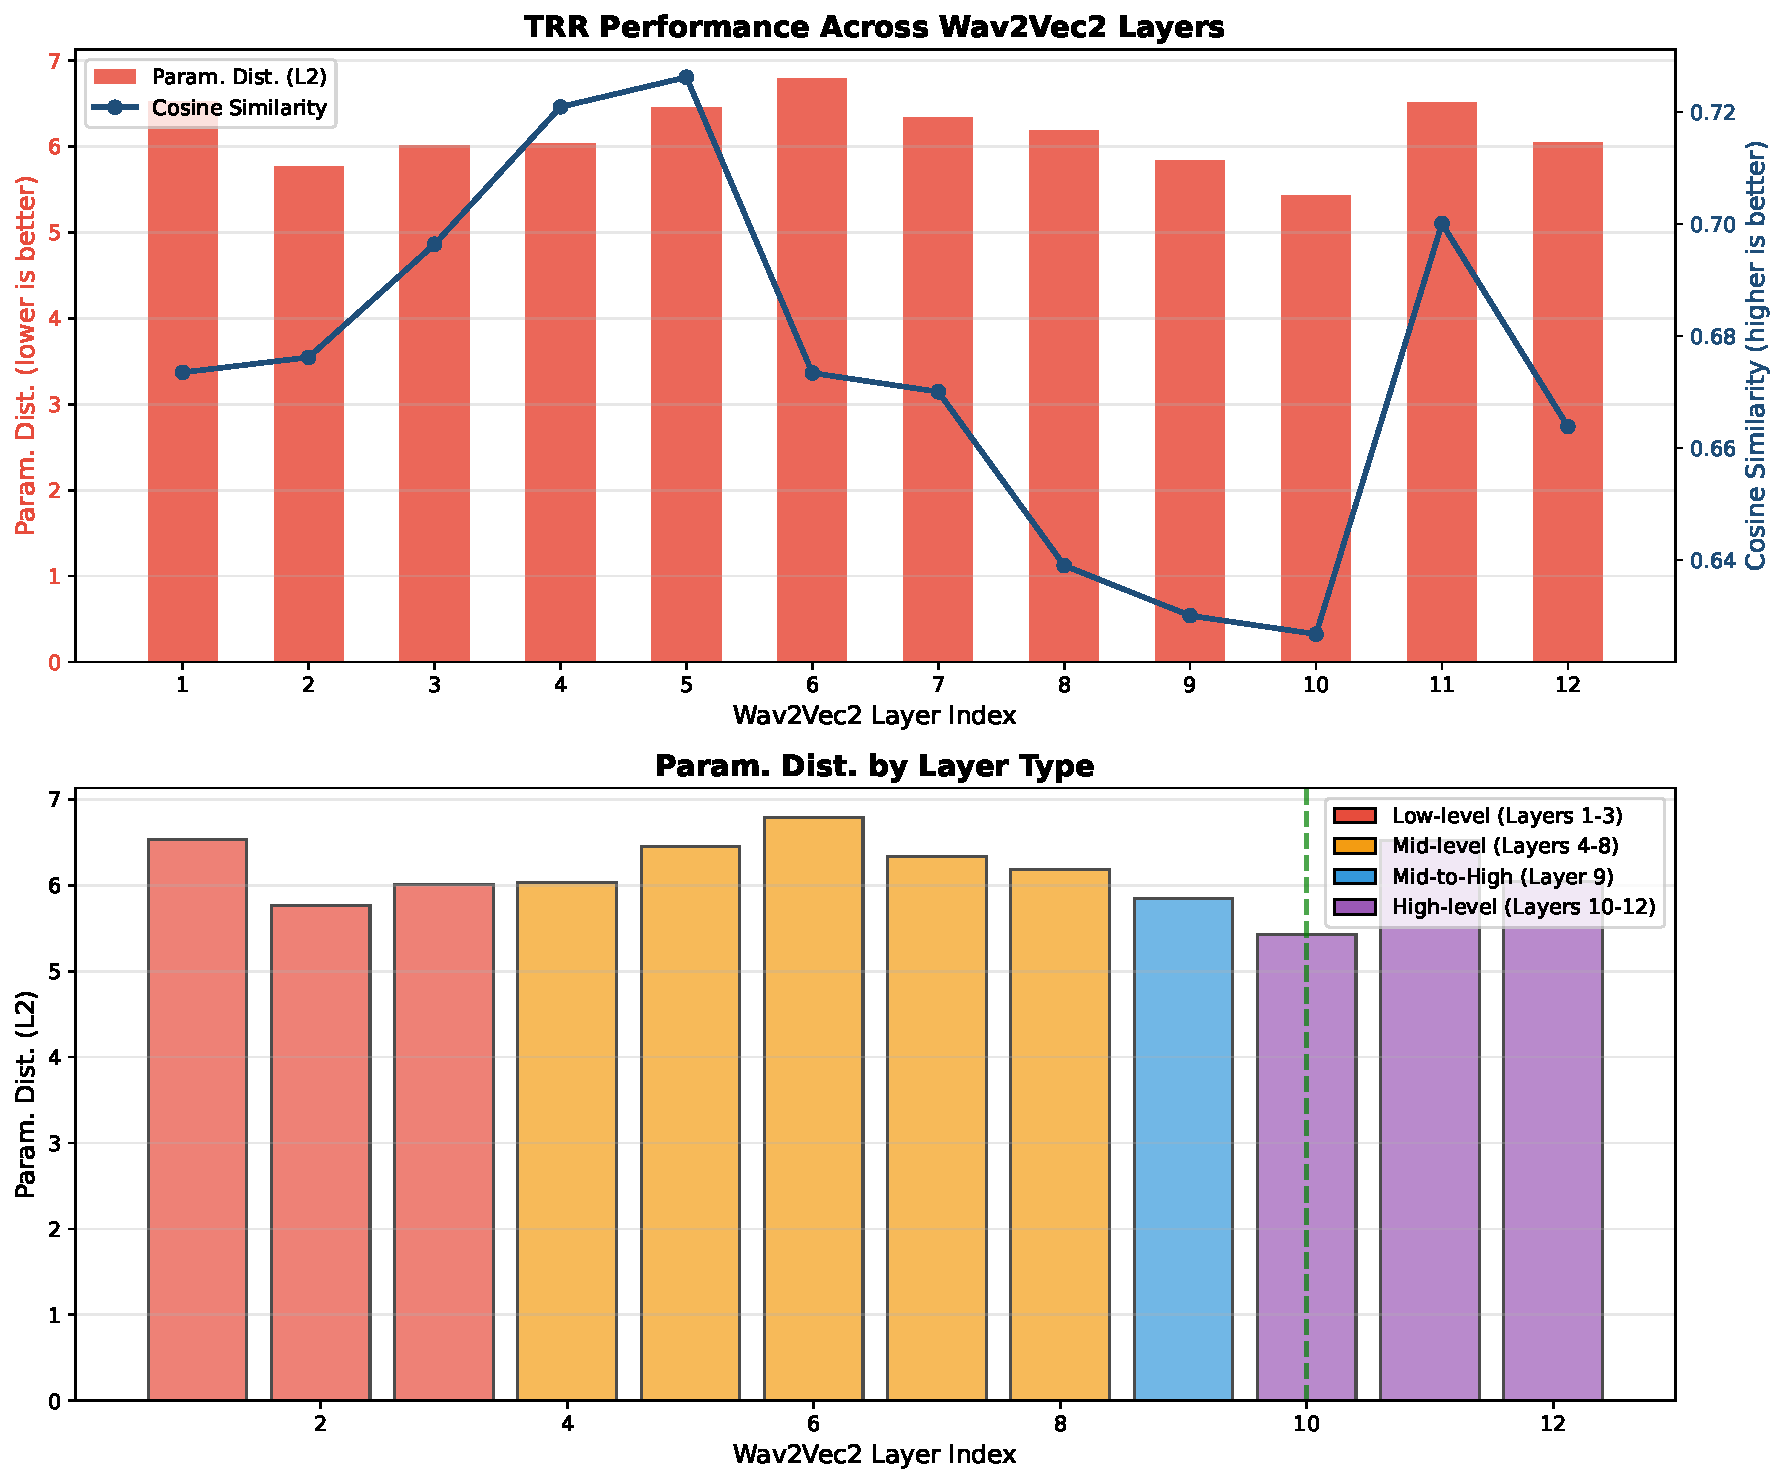
\includegraphics[width=0.82\textwidth]{trr_layer_selection.pdf}
\caption{TRR mechanism and layer-selection diagnostic from the 204-query P0 mechanism artifact. The plot provides bounded evidence about which Wav2Vec2 layer region and aggregation choice give the most useful texture representation under the current benchmark.}
\label{fig:trr_layer_selection}
\end{figure*}

\begin{figure*}[t]
\centering

\includegraphics[width=0.86\textwidth]{per_param_error_dist.pdf}
\caption{Per-parameter error distribution diagnostic. The figure complements the aggregate Protocol-A/Protocol-B metrics by showing where normalized parameter errors concentrate across effect-chain leaves.}
\label{fig:per_param_error_dist}
\end{figure*}

The diagnostics are consistent with the bounded mechanism interpretation used in the supplementary material. Same-backbone Gram aggregation improves over mean pooling in the archived and local mechanism checks, but the gain is partly entangled with mid-level layer choice and projection dimension. For this reason, the paper claims TRR as a useful texture-aware retrieval prior, not as a globally optimized audio representation family. The per-parameter view also makes clear that a lower aggregate normalized distance does not eliminate localized weaknesses: switch-like structures, sparse effect leaves, and parameters with nonlinear perceptual scales still require separate validity and perceptual audits.

\subsection{Robustness and Boundary Diagnostics}
\label{ssec:diagnostics}

We include compact robustness diagnostics in the main paper and move full sweeps, confidence intervals, EPR sensitivity, validity repair rates, and listening-test tables to the supplementary material. First, CLAP has partial coverage in the unified benchmark. On the 173-query shared subset where every retrieval prior has query and candidate vectors, TRR remains best on top-1 normalized distance (0.1487), PNR@5 (0.8150), and EPR-K5 normalized distance (0.1328). Second, near-duplicate filtering confirms that TRR remains the best full-coverage row as database density decreases, although absolute error rises as the candidate pool shrinks. Third, parameter-cluster hard splits provide a stronger stress test in which query clusters are removed from the database. TRR remains the lowest-error full-coverage row at all tested thresholds; CLAP is competitive on its covered subset but has fewer evaluable hard queries.

\begin{table}[t]
\centering
\caption{Compact robustness diagnostics. Near-duplicate rows report TRR normalized L2 after removing candidates within the threshold of any query. Hard-split rows report the best full-coverage TRR normalized L2 under parameter-cluster exclusion. Full baseline sweeps and confidence intervals are provided in the supplementary material.}
\label{tab:robustness_summary}
\small
\setlength{\tabcolsep}{4pt}
\resizebox{\columnwidth}{!}{%
\begin{tabular}{lccc}
\toprule
\textbf{Diagnostic} & \textbf{Setting} & \textbf{KB / $n_q$} & \textbf{TRR Norm.L2} \\
\midrule
No filter & threshold 0.000 & 1063 / 204 & 0.1454 \\
Near-duplicate filter & threshold 0.010 & 342 / 204 & 0.1968 \\
Near-duplicate filter & threshold 0.020 & 151 / 204 & 0.2510 \\
Hard split & $\tau_{\mathrm{cluster}}=0.01$ & 278 / 50 & 0.2065 \\
Hard split & $\tau_{\mathrm{cluster}}=0.02$ & 142 / 46 & 0.2424 \\
Hard split & $\tau_{\mathrm{cluster}}=0.05$ & 117 / 38 & 0.2668 \\
\bottomrule
\end{tabular}
}
\end{table}

Figure~\ref{fig:robustness_result_curves} plots the same robustness evidence as curves. The near-duplicate panel shows that TRR degrades as candidate density is reduced, but remains the strongest full-coverage row through the reported thresholds. The hard-split panel shows the expected increase in error when parameter clusters are excluded from the database; this is a stress-test result rather than a production setting. The figure is generated from the existing E9 robustness artifacts and is included to make the degradation trend inspectable in the main paper.

\begin{figure*}[t]
\centering

\includegraphics[width=0.94\textwidth]{robustness_result_curves.pdf}
\caption{Robustness result curves from the existing E9 artifacts. Left: near-duplicate removal sensitivity. Right: parameter-cluster hard-split sweep with bootstrap confidence intervals where available. Lower normalized L2 is better.}
\label{fig:robustness_result_curves}
\end{figure*}

The direct-regression boundary and Protocol-B diagnostics further delimit the claim. The range-projected MLP row in Table~\ref{tab:main_results} nearly matches TRR EPR-K5 on normalized tolerance, but it is weaker on normalized distance, recall, and cosine similarity and has no retrieved-neighborhood provenance. TRR top-K retrieval reaches PNR@5=0.7500 on the 204-query Protocol-A split, and TRR EPR-K5 is the primary hybrid result with $N_{\mathrm{eff}}=4.2129$ and $\max_i w_i=0.3438$. Figure~\ref{fig:epr_sensitivity_result_curve} summarizes the EPR sensitivity artifact: increasing $K$ improves normalized distance but also spreads provenance over more exemplars. We therefore report K5 as the main hybrid operating point because it improves over top-1 while retaining a compact neighborhood. A module-aware reranking diagnostic is negative in this run, increasing Norm.L2 by 0.0024 and decreasing Recall and Cosine; it is therefore not reported as a gain.

\begin{figure*}[t]
\centering

\includegraphics[width=0.94\textwidth]{epr_sensitivity_result_curve.pdf}
\caption{Protocol-B EPR sensitivity from the existing E9 artifact. Left: normalized L2 as a function of K, weighting, and softmax temperature. Right: effective exemplar count, showing the provenance-spread trade-off. The dashed line marks the K5 operating point used in the main table.}
\label{fig:epr_sensitivity_result_curve}
\end{figure*}

\subsection{Degraded-Input and Listening Diagnostics}
\label{ssec:supp_diagnostics}

We also surface two diagnostic groups that were previously only summarized textually. First, degraded-input fusion re-encodes waveform degradations (AWGN, MP3, reverberation, and truncation) before retrieval. The best adaptive fusion setting obtains L2=20.1491, Acc@0.1=0.6121, MRR=0.5654, and NDCG@5=0.5566, but its margin over strong fixed text-weighted fusion is small. Figure~\ref{fig:fusion_weight_distribution} shows the learned weight distribution used to inspect whether the adaptive policy collapses to a single modality or distributes mass across retrieval cues. Figure~\ref{fig:fusion_failure_analysis} then breaks down the failure cases in the uncertainty space and by modality distance. Together, these figures support the boundary statement that adaptive fusion is a robustness diagnostic rather than a primary contribution.

\begin{figure}[t]
\centering
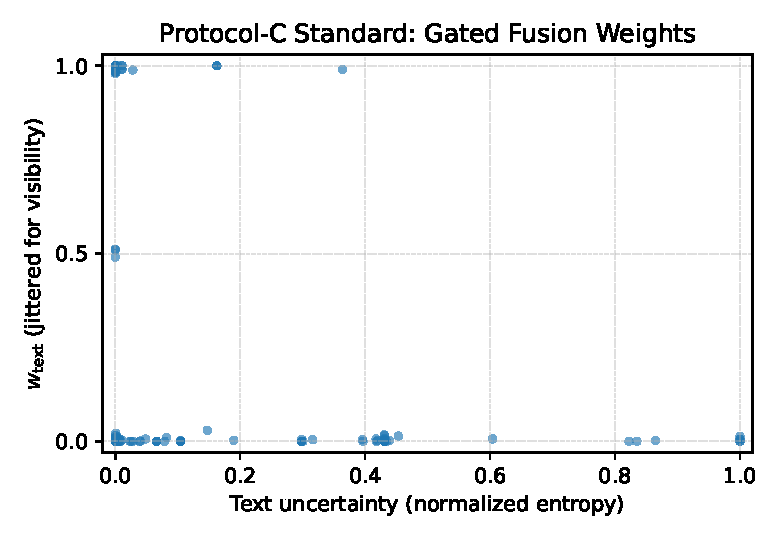
\includegraphics[width=0.92\linewidth]{fusion_weight_distribution.pdf}
\caption{Fusion-weight distribution diagnostic for the degraded-input fusion experiment. The adaptive policy is retained as boundary evidence because its margin over strong fixed text-weighted fusion is small.}
\label{fig:fusion_weight_distribution}
\end{figure}

\begin{figure*}[t]
\centering

\includegraphics[width=0.92\textwidth]{fusion_failure_analysis.png}
\caption{Fusion failure-case analysis. The diagnostic plots inspect where adaptive fusion fails or succeeds in uncertainty space, category counts, and modality-distance comparisons. It is used to delimit robustness behavior rather than to claim a dominant fusion strategy.}
\label{fig:fusion_failure_analysis}
\end{figure*}

Second, a 26-participant multiple-stimulus listening study provides perceptual context. Figure~\ref{fig:listening_trial1} shows the Trial~1 style-matching distribution, Figure~\ref{fig:listening_trials2_5} shows the manual-baseline comparison trials, and Figure~\ref{fig:listening_trials6_10} shows the MusicGen comparison trials. The observed distributions support a cautious interpretation: the TRR-based system is competitive in the tested listening setup, but the study is not a standard MUSHRA protocol and does not validate the objective metrics as human-rating proxies.

\begin{figure*}[t]
\centering

\includegraphics[width=0.94\textwidth]{system_boxplot_Trial_1.png}
\caption{Listening-study Trial~1 score distribution for style matching. This is supporting perceptual context rather than the primary validation protocol.}
\label{fig:listening_trial1}
\end{figure*}

\begin{figure*}[t]
\centering
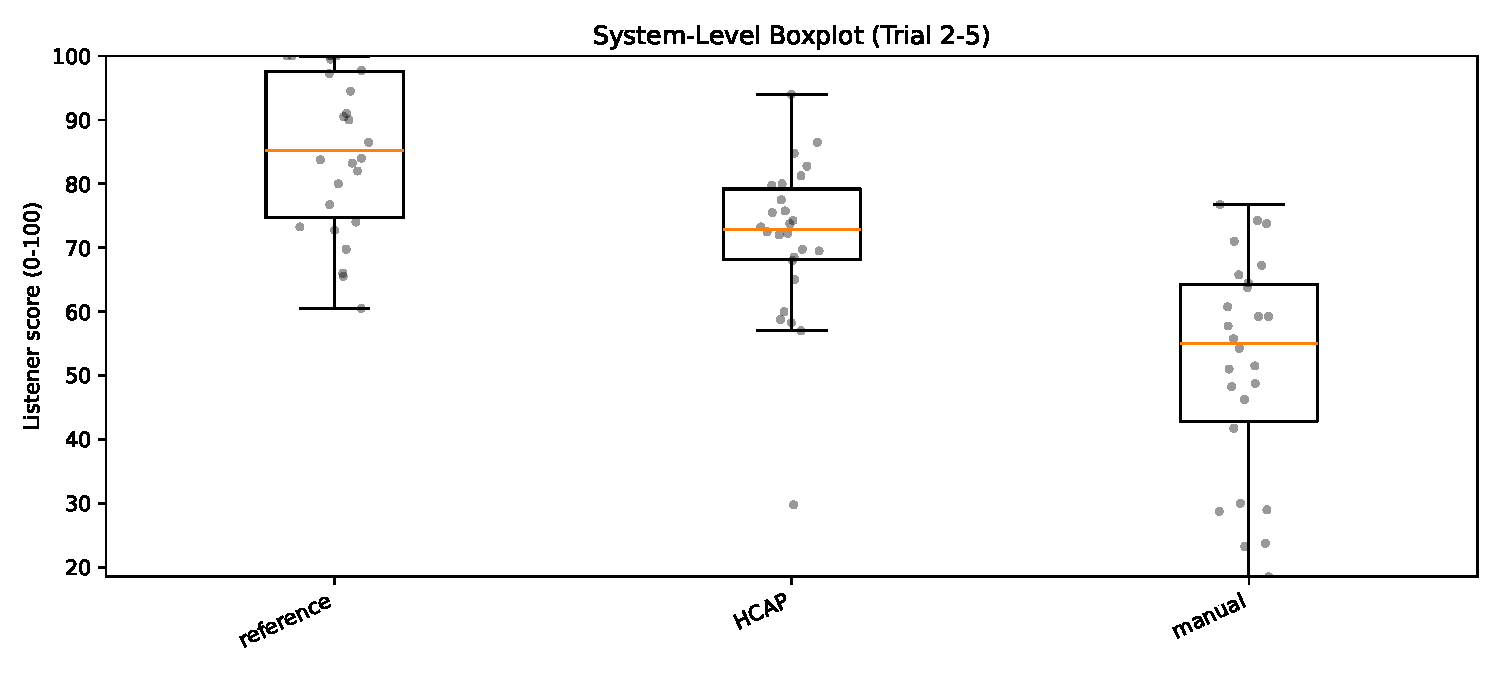
\includegraphics[width=0.94\textwidth]{system_boxplot_Trial_2_5.pdf}
\caption{Listening-study Trials~2--5 score distributions comparing the TRR-based system with a manual baseline. The study is treated as supporting perceptual context rather than as the primary validation protocol.}
\label{fig:listening_trials2_5}
\end{figure*}

\begin{figure*}[t]
\centering

\includegraphics[width=0.94\textwidth]{system_boxplot_Trial_6_10.png}
\caption{Listening-study Trials~6--10 score distributions comparing the TRR-based system with MusicGen. The figure supports a parity-style interpretation rather than a superiority claim.}
\label{fig:listening_trials6_10}
\end{figure*}

Because the listening study lacks a standard low-quality anchor, device metadata, participant-expertise labels, and a documented manual-tuning time budget, we treat it as supporting context rather than a primary validation of Protocol-A or Protocol-B. A metric--perception alignment diagnostic is also negative under the available alias mapping. Together, these results reinforce that the main claim is parameter-space transferability under audited retrieval protocols, not a validated predictor of human listening scores.

\section{Discussion}
\label{sec:discussion}

\subsection{Scope of the Current Evidence}
\label{ssec:memory_exp}

The core quantitative evidence is the unified Protocol-A/Protocol-B retrieval and projection benchmark on a 204-query guitar-only split, supplemented by near-duplicate sensitivity, CLAP-covered shared-subset analysis, EPR sensitivity, EPR validity/repair auditing, mechanism ablations, and the supervised direct-regression boundary. Protocol-C and the listening/local-vLLM diagnostics provide additional stress-test and perceptual characterization. All claims about texture-aware retrieval are bounded to this benchmark; generalization to other instruments, effect families, or production stages is hypothesized but not validated. Personalization and memory components are outside the paper's validated claims because they are not evaluated under the same held-out protocol.

\subsection{Implications for Audio Effect Control}

The current results suggest a practical pattern for retrieval-based audio control: use retrieval over real presets to provide feasibility constraints and stylistic priors, and then expose the retrieved configuration for direct user editing. In Protocol-A, TRR achieves the strongest parameter alignment among the full-coverage retrieval rows while preserving editability and traceability in DAW workflows. Protocol-B sharpens the boundary: MLP+RangeProjection is a direct-regression baseline, while EPR-K5 is the strongest hybrid result when executable-neighborhood provenance is part of the target. Together, these results support TRR as a retrieval prior with measurable parameter-transferability benefits on this benchmark.

\paragraph{Retrieval versus regression.} The MLP boundary clarifies the fundamental trade-off between retrieval-based and regression-based approaches. On Norm.Acc@0.1, MLP (0.7894) is effectively tied with TRR EPR-K5 (0.7908): the gap of 0.0014 is well within sampling variability. However, on Recall the gap is large (0.3468 vs.\ 0.7146), indicating that the MLP regressor fails to activate the same set of parameters as ground truth even when its numeric values are within tolerance on the dimensions it does predict. Similarly, Cosine similarity (0.5941 vs.\ 0.9207) shows that the MLP's predicted parameter vector is structurally misaligned with ground truth. The retrieval approach succeeds because it anchors predictions to real preset exemplars: every retrieved parameter is drawn from an executable neighborhood, so the output inherits the activation patterns and correlations of real presets. Regression, by contrast, produces point estimates that may be numerically close on individual parameters but lack the global structure of valid presets. This trade-off---numerical precision versus provenance and structural alignment---is the central design rationale for TRR: the system is not primarily motivated by tolerance accuracy, but by the ability to produce outputs that are structurally coherent, editable, and traceable to specific exemplars.

\paragraph{Stakeholder considerations.} Different user groups may experience the system differently. Amateur guitarists may value one-click preset retrieval and simple top-1 selection, whereas professional session musicians and sound designers may prefer browsing a top-$K$ gallery or inspecting the provenance weights of an EPR-K5 blend. Mixing engineers care about how a retrieved guitar tone sits in a full mix, a perspective not captured by isolated parameter-space metrics. Plugin developers must weigh the storage and latency costs of a retrieval index against the benefits of semantic search. The current evaluation does not distinguish these stakeholders; future HCI work should conduct task-based studies with representative user groups to assess whether retrieval-based control improves workflow efficiency and creative satisfaction.

\subsection{Revisiting the Texture Hypothesis}

In Protocol-A, TRR improves parameter-space alignment over the mean-pooled Wav2Vec baseline. This comparison controls for the acoustic backbone and changes the aggregation operator from first-order pooling to second-order Gram statistics. The supplementary mechanism ablation reinforces this interpretation: on the same 204-query split, a same-layer Gram representation improves normalized L2 over mean pooling, the full unprojected Gram boundary also improves over mean pooling, and removing L2 normalization degrades retrieval quality. It therefore supports the hypothesis that correlation structure can be useful as a texture descriptor for retrieval.

We note an important caveat: the backbone-controlled comparison changes both the aggregation operator (mean pooling $\rightarrow$ Gram matrix) and the feature processing pipeline (single-layer final representation $\rightarrow$ multi-layer mid-level projection). The supplementary ablation (Table~S5) now includes a same-layers mean-pooling baseline: mean-pooling across layers~4--6 improves only marginally over mean-pooling layer~5 alone (0.2552 vs. 0.2582), and multi-layer Gram with $d=64$ improves only marginally over multi-layer mean pooling (0.2546 vs. 0.2552). The clearest Gram advantage appears on single-layer~5 (0.2457 vs. 0.2582). The gain is therefore consistent with the texture hypothesis but not experimentally isolated from mid-level layer selection: the advantage could reflect the suitability of layer~5 for this benchmark as much as the superiority of Gram statistics over mean pooling. We frame TRR as a useful texture-aware retrieval prior rather than as proof that Gram statistics alone are sufficient.

The derived per-query analysis further characterizes where TRR matters most: texture-aware correlation structure is especially beneficial when coarse semantic similarity alone is insufficient and retrieval depends on texture-specific co-activation patterns. The ablation shows that layer selection and projection dimension are not cosmetic details; the reported implementation is a practical operating point. We interpret TRR as a retrieval prior for texture-sensitive control that complements first-order semantic representations.

An open direction is whether analogous second-order representations transfer to other audio-effect settings beyond the current benchmark, including additional instruments, effect families, and mix-stage tasks. Future work can validate this through controlled cross-domain protocols and human preference judgments.

\subsection{Ethical Considerations}

The current retrieval-grounded system is intended to augment user creativity rather than replace it. Risks include homogenization toward common exemplar neighborhoods and over-reliance on suggested settings. We examined the genre distribution of retrieved presets and found no evidence of extreme bias toward a single dominant style, but the corpus itself is guitar-centric and may underrepresent niche genres. In future deployments, the interface should emphasize transparency (e.g., showing retrieved references) and user agency (e.g., direct editability and opt-out of retrieval). More generally, any model or retrieval corpus built from existing recordings or presets should consider copyright, licensing, and data provenance constraints.

\section{Limitations}
\label{sec:limitations}

Our approach has several limitations that matter directly for how the present evidence should be interpreted:
\begin{itemize}
	\item \textbf{Scale and coverage.} The objective benchmark is a 204-query, guitar-only split with a single effect-chain topology. Resolved-audio grouping removes exact cross-split reuse, but cheap near-duplicate risk and database-density dependence remain. Larger multi-instrument and multi-effect benchmarks are required before making general retrieval-framework claims.
	\item \textbf{Perceptual validation gap.} Normalized L2 improves comparability across heterogeneous parameter ranges, but it is not a perceptual normalization. Logarithmic, dB, and plugin-specific nonlinear controls can make equal normalized errors sound unequal, and the current metric--perception diagnostic does not validate the objective metrics as human-rating proxies. The listening study was not conducted as a standard MUSHRA test and lacks device metadata, participant-expertise labels, a documented manual-baseline time budget, and query-aligned ratings for the Protocol-A retrieval rows. We therefore do not claim that parameter-space improvements translate directly to perceptual improvements.
	\item \textbf{Baseline boundary.} CLAP, PaSST, and same-backbone ablations strengthen the retrieval comparison, but PANNs remains a runtime blocker in the current Python 3.12 environment. We report results only for encoders that pass the vector coverage gate in the current artifact. MLP+RangeProjection serves as a direct-regression boundary. On Norm.Acc@0.1, MLP (0.7894) is effectively tied with TRR EPR-K5 (0.7908; $\Delta=0.0014$), indicating that the TRR advantage on tolerance accuracy is small: a supervised regressor can achieve comparable parameter-level tolerance. The TRR advantage over MLP is concentrated on Recall (0.7146 vs.\ 0.3468), Cosine (0.9207 vs.\ 0.5941), Norm.L2 (0.1334 vs.\ 0.1603), and retrievable provenance. This pattern implies that TRR's core value is not primarily on tolerance accuracy---where regression is competitive---but on structural alignment, activation coverage, and exemplar traceability. EPR-K5, as a hybrid projection over retrieved exemplars, further improves over the MLP baseline across all reported metrics in Protocol-B.
	\item \textbf{Projection validity.} EPR-K5 is not pure preset retrieval: it synthesizes a projected parameter vector from retrieved exemplars. The validity audit shows that the post-projection outputs satisfy the checked finite/range/switch constraints, but the nontrivial repair rates mean the constraint projection is part of the method and must be retained in deployment.
	\item \textbf{User-centered evidence.} The paper evaluates retrieval quality via parameter-space metrics but provides no task-based user study of DAW workflow efficiency, creative satisfaction, or interface usability. Claims about ``editable starting points for DAW workflows'' are technically grounded but not validated with real users.
	\item \textbf{System scope.} Personalization, memory, and adaptive fusion are not validated under the same standard as Protocol-A. Protocol-C shows that degraded-input robustness depends on modality weighting, but the adaptive margin over strong fixed weights is small and should remain diagnostic.
	\item \textbf{Deployment cost and database dependence.} TRR adds Wav2Vec2 feature extraction and $O(D^2T_{\text{frm}})$ Gram construction after projection. Caching and approximate indexing can reduce this cost, but live deployment and out-of-distribution database expansion require separate evaluation. The uncached latency path for newly supplied reference audio is not verified in the current artifact.
\end{itemize}

These limitations define the scope of our current claims. The strongest evidence is that texture-aware correlation structure provides a useful retrieval prior for editable preset selection on this benchmark. Protocol-C further shows that degradation robustness is sensitive to fusion design. Extending the evidence base to perceptual proxies, user-centered validation, larger-scale personalization, and robust deployment is left to future work.

\section{Conclusion}
\label{sec:conclusion}

We presented parameter-transferability-aware executable neighborhood retrieval for editable guitar-effect preset selection and identified Texture Resonance Retrieval (TRR) as the strongest full-coverage retrieval representation in the unified local comparison. Across objective metrics in Protocol-A/Protocol-B (Table~\ref{tab:main_results}), TRR improves parameter alignment over Wav2Vec, FeatureNN, and PaSST, and EPR-K5 improves the TRR retrieval prior while retaining neighborhood provenance. These results support the utility of texture-aware retrieval as a prior for executable preset selection on this benchmark.

Taken together, the Protocol-A and Protocol-B evidence supports a practically relevant conclusion: retrieval over executable presets provides editable starting points for DAW workflows, mid-level texture-aware feature representations improve retrieval over selected first-order baselines on the audited guitar-effect preset benchmark, and exemplar-preserving projection improves numeric alignment while retaining provenance after explicit validity projection. The degradation, listening, local-LLM, module-aware reranking, PANNs runtime-blocker audit, and supervised-regression diagnostics provide complementary boundary characterization.

Looking forward, the most important next steps are to evaluate executable direct parameter-regression and reranking baselines, expand the degradation and listening protocols, and test whether the same retrieval and fusion advantages transfer beyond guitar effects to broader production parameter spaces such as mixing and mastering workflows.

Overall, these results support texture-aware retrieval as a useful prior for editable guitar-effect preset selection on the current benchmark. Natural next directions include evaluating the framework on broader instrument classes and effect families, integrating personalization and memory components, and validating the approach under more diverse production workflows.


\begingroup
\sloppy
\raggedright
\IfFileExists{./reference.bib}{\bibliography{reference}}{\bibliography{Paper/reference}}
\bibliographystyle{\paperbibliostyle}
\endgroup

\end{document}
